%File: formatting-instruction.tex
\documentclass[letterpaper]{article}
\usepackage{aaai}
\usepackage{times}
\usepackage{helvet}
\usepackage{courier}
\usepackage{graphicx}
\usepackage{hyperref}
\frenchspacing
\setlength{\pdfpagewidth}{8.5in}
\setlength{\pdfpageheight}{11in}
\pdfinfo{
/Title (Automatically Extracting Emotional Affect from Story Elements to Classify Interestingness)
/Author (Layla Martin, Josephine Rutten)}
\setcounter{secnumdepth}{0}  
 \begin{document}
 
\title{Automatically Extracting Emotional Affect from Story Elements to Classify Interestingness}
\author{Layla Martin \and  Josephine Rutten \\
Reykjavik University \\ \{layla16, josephine16\} @ ru.is }

\maketitle
\begin{abstract}
\begin{quote}
Interestingness is one of the key aspects of stories, yet, the community of \textit{Intelligent Narrative Technologies} has tremendous issues automatically building interesting stories, or even determining whether a story will be perceived as interesting. We assume that emotion can be used as a notion of interestingness. We therefore compared the emotions in interesting fairytales to fairytales which have been altered upfront. To extract emotions from given text, we use the EmoLex dataset, which stores boolean values for eight emotions and positive/negative, and calculate the average emotions on a per-sentence basis. We paid attention to making the database reusable for future work. We then used the gathered data to classify fairytales as altered/not altered. Our classification algorithm has an accuracy of 69\% with the possibility to improve even further by exchanging the source database for emotions in words. We therefore assume that our approach can be implemented to select interesting stories from a set of fairytales. 
\end{quote}
\end{abstract}

\section{Introduction}

Research in the field of \textit{Intelligent Narrative Technologies} focuses on automatically generating narratives for interactive games, but the algorithms neither guarantee an interesting story nor are they able to assess if a story is interesting \cite{Riedl}, yet, this evaluation is deemed crucial \cite{rowe2009storyeval}. Though the term ``interesting'' itself is highly subjective, we assume that similar readers/users have a similar understanding of interestingness, making it possible to build interesting stories for a specific group. 

We assume that emotional affect can be used to build a notion of interestingness. Elliott mentioned that ``explicit presence of a human emotion [ \dots] is necessary, and sufficient to yield storiness'' \cite{elliott}. There are several different basic emotions, Plutchik defined the eight basic emotions to be happiness, sadness, fear, anger, surprise, disgust, anticipation and trust \cite{plutchik1980emotion}. 

Our prototype is able to classify text input as ``altered'' or ``not altered'' based upon the similarity of the patterns emotion intensity follows. We assume that our alterations to the fairytales make them less descriptive and therefore less interesting. 

In the following, we will describe the problem we address, lay out related work, give a proposed approach (divided in the sub-problems emotion representation and our evaluation of classification techniques), evaluate and discuss our approach, give ideas for future work, and conclude our findings. 

\section{Problem Formulation}

Our problem consists of four essential components, two algorithms and two databases: 
\begin{itemize}
\item \textsc{Word Emotion Database}: This Java Hash Table maps words with emotions and is based upon the EmoLex dataset \cite{Mohammad}.
\item Algorithm to read emotions from text: This algorithm takes a story as input and writes the representation of it to the \textsc{Text Emotion Database} using the data from the \textsc{Word Emotion Database}.
\item \textsc{Text Emotion Database}: This database maps \texttt{text-ID} and \texttt{sentence-ID} to the average emotion intensity for every emotion in the model of \cite{plutchik1980emotion}.
\item Similarity analysis algorithm: This algorithm takes the representation of one text (from the \textsc{Text Emotion Database}), builds up an even higher aggregate representation based on approx. 80 features and compares it to other texts. We use a set of different algorithms to classify the text as ``altered'' or ``original''.
\end{itemize}

\noindent Every of these items can be individually evaluated to show its functionality. Additionally, we will evaluate the accuracy of different classification algorithms for the Similarity Analysis. Our approach can be deemed successful if the accuracy is higher than for OneR. 

\section{Related Work}
Our work builds up on the findings of story generation, story evaluation and sentiment mining. 

There are several approaches to automatically create story content available. Yet, none of these is able to automatically decide whether or not the generated story is perceived interesting. Our approach will build on top of this and allow to classify whether or not a story is interesting.

\citeauthor{Riedl} developed an algorithm which allows to generate stories in which characters are perceived ``believable''. Yet, they explicitly state that their approach does not have a computational definition of interestingness \cite{Riedl}. 

In Fa\c{c}ade the algorithm selects the best of several possible successive story beats, yet, they do not specifically focus on interestingness of the story, but rather on how to remain with a believable story though having user input \cite{Mateas}. 

\citeauthor{rowe2009storyeval} describe the need for an evaluation of the generation of narratives and set up an framework to evaluate the narrative. This evaluation is not automated \cite{rowe2009storyeval}.

There have been several ideas on how to make stories interesting: \citeauthor{swartjes} used knowledge from improvisational theatre and assume that autonomous characters should get directives on how to act to make stories interesting \cite{swartjes}. We do not use autonomous characters, but evaluate entire stories generated by most likely only one generator. \citeauthor{ware} used conflict to model interestingness in stories. They presented a pseudocode algorithm for generating conflict, but we do not have knowledge about an implementation \cite{ware}. 

Mohammad built a database which maps words to emotions \cite{Mohammad}. We use his data to aggregate on sentence basis. Also we use the data we generated to build a prototype similarity analysis algorithm. Yet, Mohammad did not perform any classification tasks using his dataset. 

Currently, emotion mining and sentiment analysis algorithms are predominantly applied to retrieve emotions from social media \cite{pak}, the application in the field of narratives has not been very common in the past. 

\citeauthor{Yu2003} used Na\"{i}ve Bayes with different features based on n-grams and existence of words to mine opinions from text \cite{Yu2003}. This approach is similar to ours as we also select features and then use basic algorithms though Na\"{i}ve Bayes was not among the most accurate algorithms for our application. Yet, as we are interested in emotions and interestingness rather than opinions, we cannot adapt the approach directly. 

One could also use more complex approaches such as minimum cuts in graphs as proposed by \citeauthor{pang2004sentimental} for classifying movie reviews in positive or negative. This task is slightly easier than ours, as it restricts itself to two out of eight emotions, but is similar otherwise \cite{pang2004sentimental}. Yet, we cannot use their approach as it requires tremendous amounts of training data (they used 1000 instances per class). We were not able to retrieve data for our control group but had to pre-process it ourselves. Pre-processing this large amounts of data was out of scope for this project. 
This is also the reason why we didn't use a neural network like \citeauthor{dos2014deep} used \cite{dos2014deep}. In this article, they use a deep neural network to use sentiment analysis on short text. This article jointly uses character-level, word level and sentence-level representations to perform sentiment analysis on short texts. This would be a interesting approach, but to train a neural network on text, a lot of training data is needed. In the short scope of this project, it was unattainable to alter more stories. 

\section{Proposed Approach}
To read and analyze emotions from text, we use a set of different algorithms and databases. The \textsc{Word Emotion Database} stores the emotion vector for \textasciitilde 10,000 words. The \textsc{Text Emotion Database} stores the emotion representation for texts we processed (it currently contains 60 stories). We use the generated information for the different classification algorithms. %Josephine

\begin{figure}[thpb]
      \centering
      \framebox{\parbox{3in}{
      \centering
      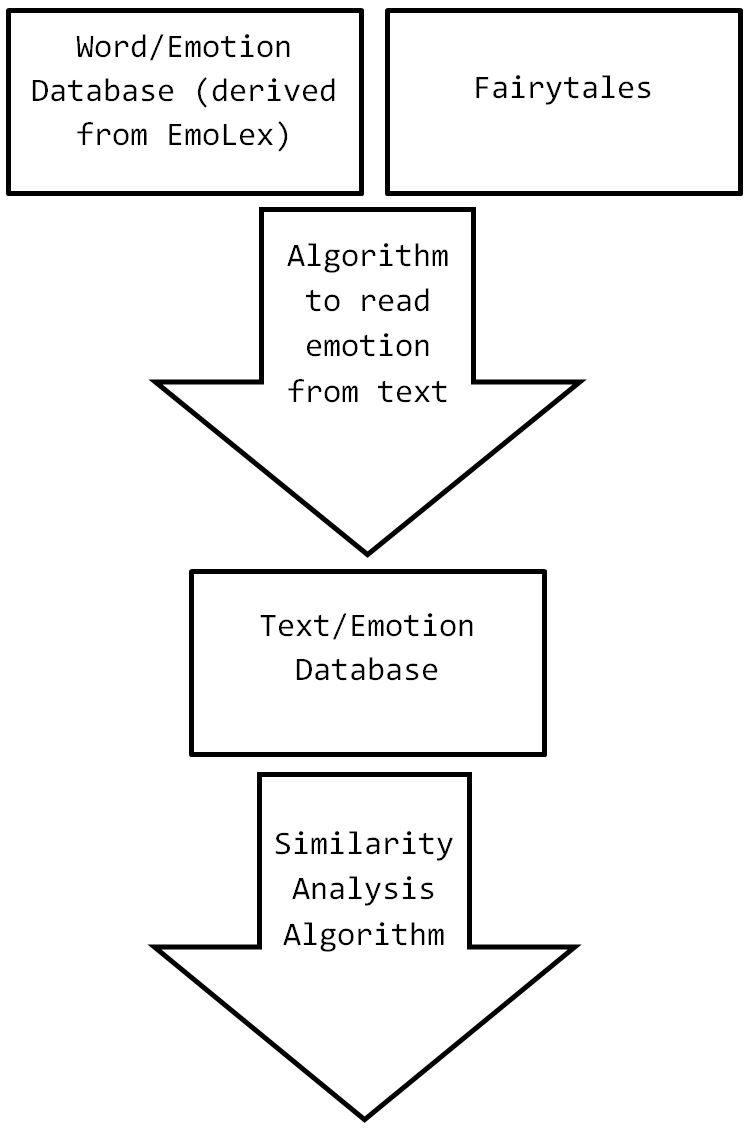
\includegraphics[width=0.35\textwidth]{images/snipINAR}}}
      \caption{Project overview}
      \label{figure:overview}
   \end{figure}

\subsection{Emotion Representation}
We need to be able to extract emotions from text and store them for future usage. To do so, we propose using a \textsc{Word Emotion Database} and a \textsc{Text Emotion Database}. In the following, we will introduce both and describe the algorithms required to fill them. 
\subsubsection{Word Emotion Database}
The \textsc{Word Emotion Database} is implemented using a Java HashMap and maps the word and boolean values for every of the eight emotions by Plutchik \cite{plutchik1980emotion} (word contains emotion or word does not contain emotion) and boolean values for positive and negative. We retrieved the data from the Mohammad et al. \cite{Mohammad}, who used Amazon Mechanical Turk to classify emotions in words. 

In the following, we will also use the notion of vectors to describe the emotions in a word. The default case being the 0-vector, if a word does not contain any information according to the EmoLex dataset or is not contained in it. 

\subsubsection{Text Emotion Database}
The \textsc{Text Emotion Database} stores the average emotions on a sentence                               . The data is stored in a MySQL database table mapping \texttt{text-ID} and \texttt{sentence-ID} as Integer values and float values for ten emotion values. 

To fill the database, we read in a fairytale and split it up into single sentences. We look up every word in a sentence in the \textsc{Word Emotion Database}. If a word is not part of the dataset, we use the zero-vector instead. We then calculate the average for every emotion and write it to the \textsc{Text Emotion Database}. 
\subsection{Classification}
With the \textsc{Text Emotion Database} given, we now need to be able to analyze the representations. In the following, we will describe how the data needs to be prepared for our similarity analysis algorithm and which data mining techniques we used. 
\subsubsection{Data Preparation}
We used the dataset from Carnegie Mellon University, which contains all fairytales by Grimm Brothers translated by Margaret Hunt \cite{carnegiemellonuniversity}. We pre-processed the data by removing line-breaks, but did not change the text otherwise. 

To test our classification algorithm, we deleted words which carry emotions but do not change the structure and meaning of the sentence. In the sentence ``Beautiful dresses, said one, pearls and jewels, said the second.'' taken from Cinderella we deleted the word ``Beautiful'' and the term ``and jewels'', yielding the sentence ``Dresses, said one, pearls, said the second.''. The representation of this sentence changes from 0.1 positive and 0.1 joy to a completely neutral sentence. We assume that these changes make the story less descriptive and therefore less interesting. 

Now Every text has a most likely unique representation in the \textsc{Text Emotion Database}, with peaks whenever a higher emotion intensity appears. As an example, figure \ref{figure:sent11} displays the emotion happiness the first fifteen sentences of the fairytale ``The Frog King''. 

\begin{figure}[thpb]
      \centering
      \framebox{\parbox{3in}{
      \centering
      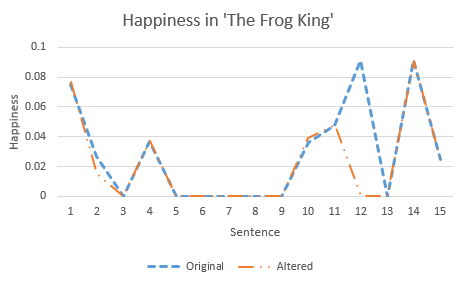
\includegraphics[width=0.4\textwidth]{images/happinessinthefrogking}}}
      \caption{Happiness of the first 15 sentences of the ``The Frog King'' before and after alteration}
      \label{figure:sent11}
   \end{figure}

As one can see, the emotion intensity highly differs from sentence to sentence, which is partially due to the differences between sentences, but also due to missing words in the EmoLex dataset and therefore our \textsc{Text Emotion Database}. 

At sentence ten the altered sentence has a slightly higher level of happiness than the original story. This sentence is somewhat special, as it contains a conversation between the frog and the princess, but no stop characters (dot). The original sentence had 81 words, while the altered sentence had 74 words. Deleting those seven words increased the ratio for the emotion happiness. 

We removed the words \textit{golden} three times and \textit{little} four times from the text. These words are both not in the EmoLex dataset. As there are still three words which contain happiness (\textit{love}, \textit{companion}, \textit{promise}), but the number of words in total decreases, the ratio increases from $\frac{3}{81}$ to $\frac{3}{74}$.

In sentence twelve the emotion happiness goes from 0.09 to 0. This is because we removed the only word that contained happiness. 

With 30 altered and 30 original fairytales with a minimum length of 30 sentences, we filled the \textsc{Text Emotion Database} and based upon that a \textsc{Text Chunk Emotion Database}, which is implemented in MySQL, too, and maps the \texttt{text-ID} with a large number of features. To allow for basic data mining algorithms, we compare three different chunks of the story, everyone consisting of ten sentences (first ten sentences, ten sentences exactly in the middle, last ten sentences). For the entire story, and every of the chunks, we calculate the maximum emotion (maximum emotion intensity over all emotions and all sentences in scope), as well as the average for every emotion (calculated from the average emotion), as denoted in the following formula with $e(w)=1$ if emotion exists and $e(w)=0$ otherwise. $S$ is the set of sentences in scope and $W_{s}$ the set of words in a sentence $s$. 

$$\frac{\sum\limits_{s \in S}{\frac{\sum\limits_{w \in W_s}{e(w)}}{\vert W\vert}}}{\vert S\vert}$$

Additionally, we calculated the same parameters for the ratio between every of the three story chunks to cater for rising or falling emotion intensity within a fairytale. 
\subsubsection{Data Mining}
As a Proof of Concept, we analyzed the data using Weka \cite{garner1995weka}. 

After testing all given algorithms in Weka, we restricted ourselves to the four best-performing ones (with respect to accuracy or number of correctly classified items), which were SMO, SGD, RandomForest and MultilayerPerceptron, and optimized these. 

Both SMO and SGD are Support Vector Machines. \cite{hotho2005brief} stated that Support Vector Machines are successful classifiers for text mining applications. 

The Weka SMO implementation built up on the results of \cite{Platt1998} and \cite{Keerthi2001}, the Stochastic Gradient Descent \cite{SGD} optimizes the parameters of a SVM using a Hinge loss function. 

To optimize SMO, we tested several different combinations of input data and got the best results for a PolyKernel (polynomial kernel function), with a logistic calibrator, and a complexity constant of 0.75. Reducing the complexity constant relative to its default value of 1 decreases the probability of overfitting, as less support vectors are used \cite[p.~224]{alpaydin2004introduction}. 

To optimize SGD, we slightly reduced the learning rate to 0.006 (rather than the default of 0.01), reducing the probability of miss an optimum, but increasing the probability of ending in a local optimum. 

We also use the Random Forest implementation of \cite{livingston2005implementation} modeled after \cite{breiman2001random}. It performs well on data with weak inputs, which is most certainly given in our case, as we pre-processed our control group only by deleting words, which might have two-fold influence on the average emotion: It can decrease if a word carrying emotion is deleted or increases if any other word is deleted, as the total number of words decreases. We do not have any means of controlling this behavior so far. 

Compared to the default settings, we switched on the parameter \texttt{BreakTiesRandomly} and reduced the \texttt{Max-Depth} parameter to 5 (compared to infinity). These settings introduce added randomness, which helps with data scarcity (ties), and reduce the probability of overfitting of the decision trees by pruning. 

Multilayer Perceptrons (MLPs) are an implementation of neural networks using feed-forward propagation \cite{rosenblatt1961principles,haykin2004comprehensive}. They consist of an input layer, hidden layers, and an output layer. 

We optimized the MLP by setting the number of hidden layers to two. The reason for a that low number is most likely the amount of pre-processing as well as the little number of stories. 

Neural Networks are iteratively optimized by applying it to the training data and adjusting the weights accordingly. The parameter training time specifies how often this procedure is executed. Figure \ref{figure:MLP} shows the number of correctly classified instances compared to training time. It got two optima at 50 and 100 iterations, but decreases again with higher training time. This can most likely be explained by overfitting. 

\begin{figure}[thpb]
      \centering
      \framebox{\parbox{3in}{
      \centering
      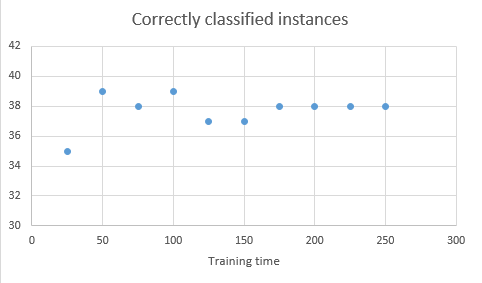
\includegraphics[width=0.4\textwidth]{images/trainingtimeneuralnetwork}}}
      \caption{Influence of Training Time on correctly classified instances of the Multilayer Perceptron}
      \label{figure:MLP}
\end{figure}

%might help: http://ieeexplore.ieee.org/document/159058/


\section{Evaluation}
As discussed earlier, every of our problem components can be evaluated individually for their functionality. The \textsc{Word Emotion Database} stores all words from the EmoLex dataset \cite{Mohammad}, they can be queried by the other components. We implemented a working algorithm to read emotions from fairytales into our \textsc{Text Emotion Database}, from where the data can be retrieved by our similarity analysis algorithm. 

In the following, we will present the results from the proposed approach and give some ideas on how to improve the results in later repetitions of the project. 
\subsection{Results}

%used algorithms
We tested the four best performing algorithms against OneR. OneR used the average anticipation in the first ten sentences (parameter \texttt{meanant1}) to build up a model. It correctly classifies 31 out of 60 elements (and therefore just slightly better than random). We used 10-fold cross validation for all algorithms where applicable.

The other algorithms correctly classify 39, 40, or 41 elements, which reflects in the accuracy given in table \ref{table:performance}. This table also shows true positive and true negative rate (TPR, TNR). 

Though SMO and SGD both build up support vector machines, and have identical accuracy, they do not build up the same classifier, as TPR and TNR differ. SGD is the best algorithm to classify altered stories (abreast with Random Forest), SMO is the best to classify unchanged stories. 

%accuracy
\begin{table}
\begin{tabular}{c|c|c|c}
algorithm & accuracy & TPR & TNR \\
\hline
OneR & 0.52 & 0.50 & 0.53 \\
\hline
MLP & 0.65 & 0.67 & 0.63  \\
\hline
SMO & 0.67 & 0.63 & 0.70 \\
\hline
SGD & 0.67 & 0.70 & 0.63 \\
\hline 
RandomForest & 0.69 & 0.70 & 0.67 \\
\end{tabular}
\caption{Classification performance of different algorithms}
\label{table:performance}
\end{table}

Random Forests perform best with respect to accuracy, correctly classifying 41 stories. But this finding cannot be easily transferred to other datasets, as this algorithm tends to behave highly random. According to \citeauthor{breiman2001random} both the items to build up the tree as well as the features which are used at a specific node are chosen at random \cite{breiman2001random}. Thus, the classification is vastly dependent on the selection of the random seed. To show this, we plotted the number of correctly classified items for different random seeds in figure \ref{figure:seedRF}. 

\begin{figure}[thpb]
      \centering
      \framebox{\parbox{3in}{
      \centering
      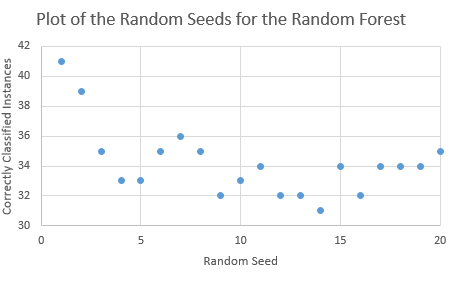
\includegraphics[width=0.4\textwidth]{images/randomtree}}}
      \caption{Influence of seed on correctly classified instances of Random Forests}
      \label{figure:seedRF}
\end{figure}

This instability also holds for MultilayerPerceptron, which does not use ten-fold cross-validation, but separates data in test and training data itself. Therefore, it is more susceptible to random influences than the support vector machines. Thus, the random seed has a higher influence. This can be seen in figure \ref{figure:seedMLP}.

\begin{figure}[thpb]
      \centering
      \framebox{\parbox{3in}{
      \centering
      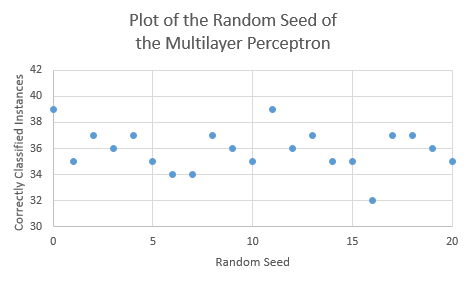
\includegraphics[width=0.4\textwidth]{images/randomseedmultiper}}}
      \caption{Influence of seed on correctly classified instances of the Multilayer Perceptron}
      \label{figure:seedMLP}
\end{figure}

We also found unexpected behavior when using different learning rates in MultilayerPerceptron, which are most likely evidence of too few data for an algorithm as complex as this one. Please refer to figure \ref{figure:learningRate} to learn how learning rate and number of correctly classified instances are related. 

\begin{figure}[thpb]
      \centering
      \framebox{\parbox{3in}{
      \centering
      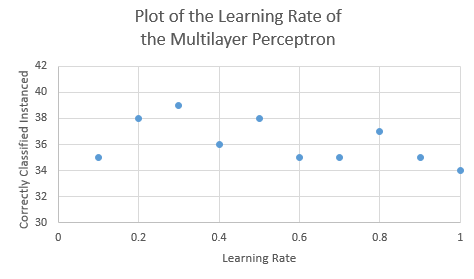
\includegraphics[width=0.4\textwidth]{images/learningrate_mlp.png}}}
      \caption{Influence of Learning Rates on correctly classified instances of the Multilayer Perceptron}
      \label{figure:learningRate}
\end{figure}

\subsection{Conceptual critique}
%problems with EmoLex dataset.
We used the EmoLex dataset by \citeauthor{Mohammad}. For a first prototype, the data is sufficient, but for more elaborate algorithms, this work needs to be repeated, as many words are not contained (e.g. \textit{greater} and \textit{greatest} are included, \textit{great} is not included). Also, \textit{greater} is deemed positive, whilst \textit{greatest} is not. In particular for fairytales, which often use older words, word stem analysis would be very helpful. Rather than having just around 10,000 words, having a larger database makes the results more reliable. Consider the following sentence of the fairytale ``Mother Holle'':

$<``Never\ an\ angry\ word.'',anger=\frac{1}{4}, anticipation=0, disgust=\frac{1}{4}, fear=0, happiness=0, sadness=0, surprise=0, positive=0, negative=\frac{1}{4}>$

Removing the word \textit{angry} with the emotions $anger=1$, $disgust=1$, and $negative=1$, whilst none of the other words is included in the EmoLex dataset \cite{Mohammad}, yields the following vector: 

$<``Never\ a\ word.'',anger=0, anticipation=0, disgust=0, fear=0, happiness=0, sadness=0, surprise=0, positive=0, negative=0>$ 

%different lengths of sentences
Furthermore, as sentences are of tremendously different length, the average emotion can be quite high if there is just a single word containing this emotion. 

Consider removing any other word than \textit{angry} in the previous example, \textit{never} for instance. The values for anger, disgust and negative increase by $33\%$ by only removing this word, though the actual emotion contained in the sentence stays the same. There is no easy approach to remedy this, taking the absolute value will privilege longer sentences over shorter ones, the average seems the most reasonable approach. 

%option: remove words which are not in the EmoLex dataset
Another alternative which we evaluated was to only consider words which are contained in the EmoLex dataset, but some sentences only consist of words which are not included, which would yield in a division by 0 when calculating the average, as the EmoLex dataset does not contain all emotion-carrying words. 

%problems with data preparation for control group
We found it rather complex to prepare the data for the control group. As described, we deleted words from sentences, which don't affect the grammatical integrity of the sentence. Yet, in several cases this has proven to be difficult. Consider the following sentence of the fairytale ``Clever Hans'': 

\textit{Hans answered, to Gretel.}

None of the words can be deleted to still retrieve a grammatically valid sentence. 

With that few training data and the previously explained random influences, accuracies of at least 25\% above OneR are sufficient. 

\section{Discussion}

With this work we have shown that it is possible to classify text as altered/unaltered using the emotion contained in the words of the text. 

Our approach to include emotions in the evaluation of stories is unprecedented. 

We used four different data mining techniques to classify text from 60 fairytales out of which half was altered. Every one of these proved to be at least 25\% better than OneR. 

We assume that our Proof of Concept can be applied in many different fields, where one has to select from different stories or story elements, as it is easy to understand and reuse. Extensions can easily be made. 

Though only being a Proof of Concept rather than a extensive solution, we assume that future work can build up on our findings to implement emotion mining techniques in story evaluation. 

%McNemar Test

\section{Future Work}

As mentioned previously, the EmoLex \cite{Mohammad} dataset does not have sufficient extent. To get more reliable results, one should repeat the work. Rather than representing emotion as a boolean value (exists or does not exist), one could introduce an amplitude (\texttt{float} value), for example in the range of -10 to +10 (contains the opposite of the emotion to contains vast amounts of emotion. With this approach, one could also address challenges such as comparison (e.g. $<good,positive,1>$, $<better,positive,2>$, $<best,positive,3>$). The words which are required for classification and therefore need to be included in the \textsc{Word Emotion Database} are dependent on the domain, and so is the annotation. In fairytales, ``witch'' is usually used in a negative manner, in modern stories for children, the witch might even be the main character. Thus, it is required to adapt the \textsc{Word Emotion Database} to the domain. 

Additionally, our prototype does not contain word stem analysis. In future work, one might address this by transforming both the words in the \textsc{Word Emotion Database} and the story and assigning them the emotion vector of the most suitable word in the database. 

Currently, our prototype does not cater for negations, we assume that building up dependency trees for semantic analysis can help. The influence of the word to which the negation relates, could be negated or the importance of this word could be lowered. 

Also, we do not care for the intention behind a sentence, a sentence ending with an exclamation mark could be deemed higher than the one ending with a question mark. These challenges should be tackled in collaboration with linguists, as the intention vastly depends on the author of the story in question. 

Our current classification algorithm is simply used to prove the possibility of using emotion to derive ``interestingness'' of text. There are several other fields of application, in which the emotion might be used to build interesting stories: If we allow users to choose the outcome of a story, we either have to author vast amounts of story content (all parts of the branching story), prune our story tree, or have to be able to assess the quality of automatically authored story content, though the quality might depend on the context. Assuming that an interesting story adheres to given patterns which can be determined upfront, select successive story chunks or beats depending on their similarity to given ``good''/interesting stories. Alternatively, given text could be annotated with required emotions to match given patterns. 


\section{Conclusions}

In this paper, we presented our prototype for classifying interestingness of stories based on the emotion in them. Our contributions include a comparison of different data mining algorithms, concluding that in particular neural networks (Multilayer Perceptron), support vector machines (SMO, SGD) and Decision Trees (Random Forests) are applicable. 

From the above results, we conclude that it in general is possible to use the emotion pattern to classify stories for their ``interestingness''. We assume that further improvement to this prototype and on the EmoLex dataset as well as increasing the training dataset will help to get even more reliable results. 

\addtolength{\textheight}{-12cm}   % This command serves to balance the column lengths
                                  % on the last page of the document manually. It shortens
                                  % the textheight of the last page by a suitable amount.
                                  % This command does not take effect until the next page
                                  % so it should come on the page before the last. Make
                                  % sure that you do not shorten the textheight too much.

\bibliography{inar}
\bibliographystyle{aaai}
\end{document}